\documentclass[12pt,a4paper]{article}
\usepackage{fancyhdr}
\usepackage{fontspec}
\usepackage{amsmath}
\usepackage{amssymb}
\usepackage{bm}
\usepackage{tikz}
\usepackage{pstricks-add}
\setmainfont{Microsoft YaHei}
\pagestyle{fancy}


\begin{document}

\newcommand{\nl}{\newline}
\newcommand{\ntinf}{\lim\limits_{n \to \infty}}
\newcommand{\xtinf}{\lim\limits_{x \to \infty}}
\newcommand{\ntx}[1]{\lim\limits_{n \to #1}}
\newcommand{\xtx}[1]{\lim\limits_{x \to #1}}
\newcommand{\ttx}[1]{\lim\limits_{t \to #1}} 
\newcommand{\ktx}[1]{\lim\limits_{k \to #1}} 
\newcommand{\dxtx}[1]{\lim\limits_{\Delta x \to #1}}
$\nl$

\begin{center}第10章 级数  \end{center}




$部分和S_n,n=1~k$

$\frac{1}{lnn}-\frac{1}{ln(n+1)}=\frac{1}{\zeta ln^2 \zeta}> \frac{1}{(n+1)ln^2(n+1)}$

$\nl$

$设\{a_n\}单调递减且非负,且级数\nsum{1}{\infty}a_n收敛,证明:\ntinf na_n=0$

$只需证明\{na_n\}的奇偶子列分别收敛于0,由Cauchy准则$

$\forall \epsilon >0,\exists N_1 \in N,当n > N时有a_{n+1},a_{n+2}...a_{2n} < \frac{\epsilon}{2} 由单调性$

$na_{2n} \le a_{n+1},a_{n+2}...a_{2n} < \frac{\epsilon}{2},即(2n) a_{2n} < \epsilon$

$(2n+1)a_{2n+1}=2na_{2n+1}+a_{2n+1} \le 2na_{2n}+a_{2n+1}< \epsilon + \epsilon$

$\nl$

$在\nsum{1}{\infty}\frac{1}{n}中去掉分母含零的项,则(\nsum{1}{\infty}\frac{1}{n})^* < {90}$

$因为(\nsum{1}{\infty}\frac{1}{n})^*=(1+\frac{1}{2}+..+\frac{1}{9})+(\frac{1}{11}+\frac{1}{19}+...+\frac{1}{99})+(\frac{1}{111}+\frac{1}{119}+...+\frac{1}{999})$

$<9^1×1+9^2×0.1+9^3×0.01$

$\nl$

$e^{\pi}与\pi ^e用(\frac{x}{lnx})'比较$

$n^{\frac{1}{n}}=1,n \to \infty$

$\nsum{1}{\infty}(e-(1+\frac{1}{n})^n)^2 < \nsum{1}{\infty}((1+\frac{1}{n})^{n+1}-(1+\frac{1}{n})^n)^2=\nsum{1}{\infty}(1+\frac{1}{n})^{2n} \frac{1}{n^2}< \frac{e^2}{n^2} $

$\nl$

$\nsuminf \frac{(n!)^2}{(2n)!} \to  \ntinf \frac{a_{n+1}}{a_n}=\frac{1}{4}<1$

$\nl$

$\nsuminf n!(\frac{x}{n}^n(x>0)) \to \ntinf \frac{a_{n+1}}{a_n}=\frac{x}{e}$

$而当x=e,则\frac{a_{n+1}}{a_n}>1,则\xtinf a_{n+1} \ne 0$

$\nl$

$\nsuminf \frac{n^2}{(2+\frac{1}{n})^n},\ntinf \sqrt[n] a_n = \frac{n^{\frac{2}{n}}}{2+\frac{1}{n}}=\frac{1}{2} < 1,故收敛$

$\nl$

$\frac{1}{2}+\frac{1}{3^2}\frac{1}{2^3}+\frac{1}{3^4}+...\frac{1}{2^{2n-1}}+\frac{1}{3^{2n}}+....$

$奇子列\ntinf \sqrt[n] a_n = \frac{1}{2},偶子列\ntinf \sqrt[n] a_n = \frac{1}{3}$

$故有\sup \ntinf \sqrt a_n = \frac{1}{2} <1$

$\nl$

$ln(1+x)=x-\frac{1}{2}x^2+o(x^2)(x \to 0)$

$a_n=\frac{1}{\sqrt n}-[\frac{1}{n}-\frac{1}{2n^2}+o(\frac{1}{n^2})]^{\frac{1}{2}}$

$故\ntinf \frac{a_n}{\frac{1}{n^{\frac{3}{2}}}}=\frac{1}{4}$

$\nl$

$P判别法:P>1,0 \le l < +\infty 收敛,P \le1,0<l \le +\infty,发散$

$\nl$

$Roabe判别法:设\nsuminf a_n 为正项级数,若 \exists N \in \bold{N},使得\forall n>N时有$

$n(\frac{a_n}{a_{n+1}}-1) \ge r > 1,则收敛,若n(\frac{a_n}{a_{n+1}}-1) \le 1,则发散$

$证明:设\forall n \in N,\frac{a_n}{a_{n+1}} \ge 1+\frac{r}{n},取p(1<p<r)则1+\frac{r}{n}>(1+\frac{1}{n})^p(n \to \infty)$

$\frac{a_n}{a_{n+1}} > (\frac{n+1}{n})^p, a_{n+1}>a_n(\frac{n}{n+1})^p 故a_2<a_1(\frac{1}{2})^p,a_3<a_1(\frac{1}{3})^p$

$推论:\ntinf n(\frac{a_n}{a_{n+1}}-1)=r,r>1收敛,r<1发散$

$\nl$

$\xtx{0+}\frac{\frac{1}{e}(1+x)^{p+\frac{1}{x}}}{x} = \xtx{0+}\frac{\frac{1}{e}e^{(p+\frac{1}{x})ln(1+x)}-1}{x} 将ln(1+x)展开为x-\frac{1}{2}x^2+o(x^2)$

$有\xtx{0+}\frac{e^{(p-\frac{1}{2})x+o(x)}-1}{x}=p-\frac{1}{2}$

$\nl$

$仅有\nsuminf sin(\pi \sqrt {n^2+k^2}),k \in N$

$原级数=(-1)^n sin\frac{k^2 \pi}{\sqrt{n^2+k^2}+n^2} 当n充分大时,成为交错级数$

$且|a_n|>|a_{n+1}|,\xtinf a_n=0$

$\nl$

$阿贝尔 1^\circ 若A \le b_m+...+b_n \le B,a_mA \le \sum_k^{\infty}a_kb_k \le a_m B$

$Cauchy凝聚判别法,若\{a_n\}单调递减非负,则\nsuminf a_n 与 \nsuminf 2^n a_{2^n}同敛散$

$记S_n=a_1+a_2+...a_n,s_k'=a_1+2a_2+....2^ka_{2^k}$

$若n<2^k,有s_n \le a_1+(a_2+a_3)+(a_4+..a_7)+...+(a_{2^k}+....a_{2^{k+1}-1})$

$\le a_1+2a_2+4a_4+....2^k a_{2k}=s_k^*$

$n>2^k,s_n \ge a_1+a_2+(a_3+a_4)+(a_5+..a_8)+...+(a_{2^{k-1}+1}+....a_{2^{k}})$

$\ge \frac{a_1}{2}+a_2+2a_4+4a_8+...+2^{k-1}a_{2^k}$

$若\nsuminf a_n 收敛,S_n有界,则\forall k \in N,必有n \in N,n> 2^k,S_k' \le 2S_n$

$\nl$

$定理(隔项比值法,刘秋生)设\nsuminf a_n 为正项级数,\{a_n\}单调递减,若$

$\frac{a_{2n}}{a_n}=p,则p<\frac{1}{2}时级数收敛,p>\frac{1}{2}级数发散$

$证明:当\xtinf \frac{a_{2n}}{a_n}=p< \frac{1}{2},则有\xtinf \frac{2a_{2n}}{a_n}=p<1,令n=2^k有$

$\ntinf \frac{2a_{2·2^k}}{a_{2^k}}=2p <1 \to \ntinf \frac{2^{k+1}a_{2^{k+1}}}{2^ka_{2^k}}=2p<1 (比值法,凝聚定理)$

$\nl$

$定理(叶志江),设f(x)正值连续[1,+\infty)单调递减 \varphi (x)在[1,+\infty)$

$上可导且单调减,且\varphi (x)>x,\forall x \in [1,+\infty)若\ntinf \frac{\varphi (x)f(\varphi (x))}{f(x)}=r$

$则当r<1时,\nsuminf f(n)收敛$

$厄耳玛可夫判别法 \varphi (x)= x+1,\varphi (x)=2x,\varphi (x)=e^x$

$\nl$

$\nsuminf (1-\frac{lnn}{n})^{2n},\exists N \in \bold N:n>N后,a_n<e^{-2lnn}=\frac{1}{n^2}$

$设\{a_n\}\{b_n\}满足e^{a_n}=a_n+e^{b_n},\forall n \in N,若\nsuminf a_n^2收敛,则b_n也收敛$

$e^{b_n}=e^{a_n}-a_n=1+a_n+\frac{1}{2}a_n^2+o(a_n^2)-a_n$

$=1+\frac{1}{2}a_n^2+o(a_n^2),故b_n \to 0(n \to \infty)$

$故e^{b_n}=1+b_n+o(b_n)=1+\frac{1}{2}a_n^2+o(a_n^2)$

$从而b_n ~ \frac{1}{2}a_n^2(n \to \infty)由比较法$

$类似的,有$

$若a_n=b_n+ln(1+a_n)且\nsuminf a_n^2 收敛,证明\nsuminf b_n 也收敛$

$\nl$

$证明:\nsuminf ln(1+\frac{(-1)^n}{n^p})敛散性$

$记a_n=\frac{(-1)^n}{n^p},b_n=ln(1+a_n),c_n=a_n-b_n,则有$

$b_n=ln(1+\frac{(-1)^n}{n^p})$

$\nl$

$例:设加括号后级数发散(括号内同号)证明原级数收敛$

$|s_{nk}-s|<\frac{\epsilon}{2},|A_{k+1}|<\frac{\epsilon}{2}$

$|s_n-s|=|s_{nk}+\isum{n_k+1}{n}-s|\le |s_{nk}-s|+|A_{k+1}|<\epsilon$

$\nl$

$设f(x)在x=0处二阶可导,\xtx{0}\frac{f(x)}{x}=0,证明\nsuminf \sqrt{n}f(\frac{1}{n})绝对收敛$

$\xtx{0+}\frac{f(x)}{x^2}=\xtx{0}\frac{f'(x)}{2x}=\frac{1}{2}\xtx{0}\frac{f'(x)-f'(0)}{x-0}=\frac{1}{2}f''(0)$

$\nl$

$设f(x)为R上连续的周期为1的函数,\jf{0}{1} \varphi (x)dx=0,f'(x) \in C[0,1]$

$记a_n=\jf{0}{1}f(x)\varphi (nx)dx,n \in N,证明:\nsuminf a_n^2收敛$

$a_n^2 \le \frac{c^2}{n^2} \Leftarrow |a_n| \le \frac{c}{n},令\phi (x)=\jf{0}{x}\varphi (t)dt$

$|\varphi(x)|=|\jf{0}{[x]}\varphi(t)dt+\jf{[x]}{x}\varphi(t)dt|=|\jf{[x]}{x}\varphi(t)dt|=|\jf{0}{x-[x]}\varphi(t)dt|$

$\le |\jf{0}{x-[x]}|\varphi(t)|dt| \le \jf{0}{1}\varphi(x)dt \triangleq M$

$又f'(x) \in [0,1],|f'(x)| \le M,\forall x \in [0,1]故有$

$a_n=\jf{0}{1}f(x)\varphi(nx)dx=\frac{1}{n}\jf{0}{1}f(x)d[\phi(nx)]$

$=\frac{1}{n}[f(x)\phi(nx)|_0^1-\jf{0}{1}\phi(nx)-f'(x)dx]$

$=-\frac{1}{n}\jf{0}{1}\phi(nx)f'(x)dx$

$|a_n| \le \frac{M N}{n}$

$\nl$

$\nsuminf \frac{1}{a_n}收敛 \iff \nsuminf \frac{n}{a_1+...a_n}收敛,a_n单调递增>0$

$\Leftarrow \frac{1}{a_n} \le \frac{n}{a_1+...a_n}$

$\Rightarrow \frac{2n}{a_1+...a_{2n}} \le \frac{2n}{a_{n+1}+...a_{2n}} \le \frac{2n}{na_n} = \frac{2}{a_n}$

$\jf{0}{+\infty}|f(x)|dx收敛 g(x)=\jf{0}{+\infty}f(t)cosxtdt 一致连续$

$|sin \frac{x^1-x^r}{2}| \le \frac{1}{2}|x^1-x^n|$

$\nl$

$例:na_n收敛,\nsuminf n(a_n-a_{n-1})收敛,证明\nsuminf a_n收敛$

$记\ntinf na_n=r,\lim \nsuminf n(a_n-a_{n-1})=S$

$令b_i=1,\sum a_k = na_n-\sum k(a_k-a_{k-1})$

$\nl$

$例:设\nsuminf \frac{a_n}{n}收敛,证明\ntinf \frac{1}{n}\sum a_k=0$

$记s_n=\sum \frac{a_k}{k},\sum \frac{a_k}{k}k=s_nn-\sum s_k$

$\frac{1}{n}\sum a_k=s_n-\frac{s_1+s_2+...s_{n-1}}{n-1}\frac{n-1}{n}再用Cauchy第一定理$

$\nl$

$f \in L^2(0,\pi),证明:不可同时有\jf{0}{\pi}|f(x)-sinx|^2dx \le \frac{3}{4},\jf{0}{\pi}|f(x)-cosx|^2dx \le \frac{3}{4}$

$证明:|sinx-cosx|^2 \le 2|f(x)-sinx|^2+2|f(x)-cosx|^2$

$且\jf{0}{\pi}|sinx-cosx|^2dx=\pi$

$\jf{0}{+\infty}sin(x^2)dx=\jf{0}{+\infty}cos(x^2)dx=\frac{\sqrt 2 \pi}{4}$

$\nl$

$求出所有在[0,+\infty)上的正值函数g(x)使得$

$\frac{1}{2}\jf{0}{x}g^2(t)dt=\frac{1}{x}(\jf{0}{x}g(t)dt)^2$

$证明:即有\frac{1}{2}g^2(x)=\frac{2}{x}(\jf{0}{x}g(t)dt)g(x)-\frac{1}{x^2}(\jf{0}{x}g(t)dt)^2$

$故\jf{0}{x}g(t)dt=(1 \pm \frac{1}{\sqrt 2})xg(x)$

$求导,\pm g(x)=(\sqrt 2 \pm 1)xg'(x)$

$令f(x)=lng(x)$

$则f'(x)=\mp (\frac{1}{\sqrt 2 \pm 1})x$

$\nl$

$判敛  \   \   \  \nsuminf \frac{(-1)^{[n]}}{n^p} \ \nsuminf \frac{sinnsinn^2}{n}$

$证:\nsum{0}{\infty}\frac{1}{n!}\nsum{0}{\infty}\frac{(-1)^n}{n!}=1(\nsum{0}{\infty}=e)$

$\nl$

$令a_n=1+\frac{(-1)^n}{n},n(a_n-a_{n+1}) \nrightarrow 0,当n \to \infty$

$\sqrt {1+\sqrt{2+\sqrt{3+...\sqrt{n}}}}< \sqrt {2^2+\sqrt{2^4+\sqrt{2^8+...\sqrt{2^{2^n}}}}}
< 2 \sqrt {1+\sqrt{1+\sqrt{1+...\sqrt{1}}}} < 4
$

$x_1=\frac{c}{2},c \in R,x_{n+1}=\frac{c}{2}+x_n^2,\{x_n\}收敛性$

$\ksum{1}{\infty}\frac{2^{\frac{k}{n}}}{n+\frac{1}{k}}=\ntinf \frac{1}{n}\ksum{1}{n}2^{\zeta_k}=\jf{0}{1}2^xdx$

$求\ntinf \frac{\ksum{1}{n}k^{\alpha +1}}{n\ksum{1}{n}k^{\alpha}}(分\le -1与>-1)$

$\nl$

$设y=f(x)(x\ge 0)为严格递增连续函数,f(0)=0,g为反函数$

$则有\jf{0}{a}f(x)dx+\jf{0}{b}g(y)dy \ge ab(a \ge 0,b \ge 0)$

$几何意义:1^\circ \ b=f(a);2^\circ \ b>f(a);3^\circ \ b<f(a);$

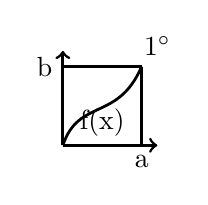
\begin{tikzpicture}[domain=1:5,line width=1pt]
\node [above] at (1.2,1) {$1^\circ$};
\draw[->]  (0,0)  --  (0,1.2);
\draw[->]  (0,0)  --  (1.2,0);

\draw  (0,1)  --  (1,1);
\draw  (1,0)  --  (1,1);

\node [below] at (1,0) {a};
\node [left] at (0,1) {b};
\node [below] at (0.5,0.6) {f(x)};

\draw(0,0)..controls (0.2,0.6) and (0.7,0.3)..(1,1);

\end{tikzpicture}

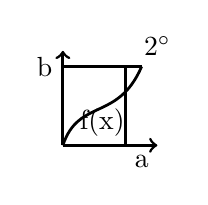
\begin{tikzpicture}[domain=1:5,line width=1pt]
\node [above] at (1.2,1) {$2^\circ$};
\draw[->]  (0,0)  --  (0,1.2);
\draw[->]  (0,0)  --  (1.2,0);

\draw  (0,1)  --  (1,1);
\draw  (0.8,0)  --  (0.8,1);

\node [below] at (1,0) {a};
\node [left] at (0,1) {b};
\node [below] at (0.5,0.6) {f(x)};

\draw(0,0)..controls (0.2,0.6) and (0.7,0.3)..(1,1);

\end{tikzpicture}

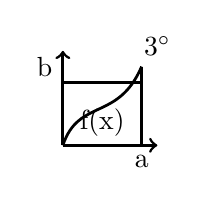
\begin{tikzpicture}[domain=1:5,line width=1pt]
\node [above] at (1.2,1) {$3^\circ$};
\draw[->]  (0,0)  --  (0,1.2);
\draw[->]  (0,0)  --  (1.2,0);

\draw  (0,0.8)  --  (1,0.8);
\draw  (1,0)  --  (1,1);

\node [below] at (1,0) {a};
\node [left] at (0,1) {b};
\node [below] at (0.5,0.6) {f(x)};

\draw(0,0)..controls (0.2,0.6) and (0.7,0.3)..(1,1);

\end{tikzpicture}
$\nl$

$arctg(k+1)-arctgk=arctg \frac{1}{k^2+k+1}$

$\nl$

$[a,b]上f(x)可积,则f(x)在[a,b]上必有无穷多个连续点$

$利用区间套证明,任取一个闭区间,存在一个连续点,而有无穷多个闭区间$

$\nl$

$f(x) \in D[0,1],|f(x)| \le \jf{0}{1}(|f(t)+f'(t)|)dt,利用分部积分$

$\jf{a}{b}fg \ge \frac{1}{b-a}(\jf{a}{b}\sqrt{fg}dx)^2,swarchy$

$\nl$

$\ntinf \frac{n}{\sqrt[n]{n!}}=e$
\end{document}

